\documentclass[UTF8]{ctexart}
\usepackage{graphicx}
\usepackage{amsmath}
\CTEXsetup[format={\Large\bfseries}]{section}
\title{机器学习——BP算法证明}
\author{学号:2011428 \\ 姓名:王天行 \\ 专业:密码科学与技术}
\date{\today}

\begin{document}
\maketitle
\clearpage

\section{作业要求}
在这个练习中,你需要以三层感知机为例,使用反向传播算法更新MLP的权重和偏置项,并将推导过程以报告的形式提交。
MLP以及权重、偏置项的定义如下:\\
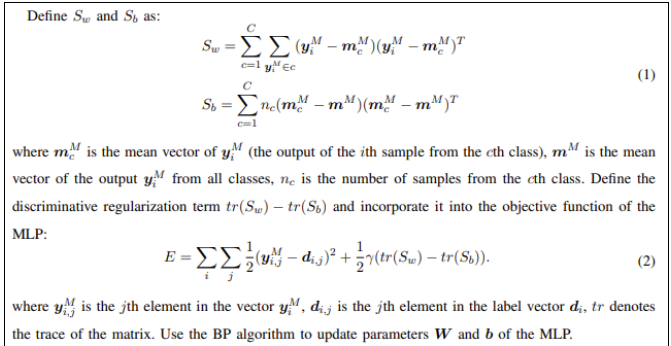
\includegraphics[width = 1\textwidth]{1.jpg}

\section{证明过程}
将MLP的输入、神经元的输出(y矩阵)和神经元的输入(n矩阵)分别视为一个矩阵,且矩阵中的一个列向量即为一个输入样本。且y和n的一行均代表所有样本对应在该神经元的输出。定义sum为输入的每个样本的特征数,p为样本数。\\
对于每一层每一个神经元,其输出 $y_{i,j}^{(l)} $为
\begin{equation}
y_{i,j}^{(l)}=\frac{1}{1+exp[n_{i,j}^{(l)}]}
\end{equation}
其中i=1,2,……,n;j=1,2,……,p\\
$y_{i,j}$ 为第j个样本的输出向量的第i个元素。对于每个神经元的输入与上一个神经元输出的关系为
\begin{equation}
n_{i}^{(l)}=\sum_{k=0}^{sum}(w_{i,k}^{(l)}\cdot y_{k}^{(l-1)}+B_{i,k}^{(l)})
\end{equation}
其中i=1,2,……,n\\
(2)式中,$B_{i,k}$ 为含有p个元素的行向量,且每个值均为 $b_{i,k}^{(l)}$ 。因此,权重项 $w_{i,j}$ 为
\begin{equation}
\begin{aligned}
\triangle w_{i,j}^{(l)}&=-\eta \frac{\partial E}{\partial w_{i,j}^{(l)}}\\
&=-\eta \frac{\partial E}{\partial n_{i}^{(l)}}\cdot \frac{\partial n_{i}^{(l)}}{\partial w_{i,j}^{(l)}}\\
&=-\eta \frac{\partial E}{\partial n_{i}^{(l)}}\cdot [y_{i}^{l-i}]^T
\end{aligned}
\end{equation}
其中i=1,2,……,n-1;j=1,2,……,n-1\\
定义 \( \delta_{i}^{l}=-\frac{\partial E}{\partial n_{i}^{(l)}} \) ,那么权重项 $b_{i,j}$ 为
\begin{equation}
\begin{aligned}
\triangle b_{i,j}^{(l)}&=-\eta \frac{\partial E}{\partial b_{i,j}^{(l)}}\\
&=-\eta \frac{\partial E}{\partial n_{i,}^{(l)}}\cdot \frac{\partial E}{\partial b_{i,j}^{(l)}}\\
&=-\eta \frac{\partial E}{\partial n_{i,}^{(l)}}\cdot I^T\\
&=\eta \delta_{i}^{(l)}\cdot R^T
\end{aligned}
\end{equation}
其中i=1,2,……,n-1;j=1,2,……,n-1;I代表全1的行向量,大小为1*n。\\
若为输出层
\begin{equation}
\begin{aligned}
\delta_{i}^{l}&=-\frac{\partial E}{\partial n_{i}^{(m)}}\\
&=-\frac{\partial E}{\partial y_{i}^{(m)}}\cdot \frac {\partial y_{i}^{(m)}}{\partial n_{i}^{(m)}}\\
&=-\frac{\partial E}{\partial y_{i}^{(m)}}\cdot S^{(m)}
\end{aligned}
\end{equation}
其中i=1,2,……,n-1;m代表输出层;矩阵$S^{(l)}$为n*n的矩阵,且只有主对角线上的元素不为0,$ S_{k,k}^{(l)}=y_{i,k}^{(l)}\cdot [1-y_{i,k}^{(l)}] $\\
若不为输出层
\begin{equation}
\begin{aligned}
\delta_{i}^{l}&=-\frac{\partial E}{\partial n_{i}^{(l)}}\\
&=-\sum_{k=0}^{sum-1}\frac{\partial E}{\partial n_{k}^{(l+1)}}\cdot \frac{\partial n_{k}^{(l+1)}}{\partial n_{i}^{(l)}}\\
&=\sum_{k=0}^{sum-1}\delta_{k}^{(l+1)}\cdot \frac{\partial n_{k}^{(l+1)}}{\partial n_{i}^{(l)}}\\
&=\sum_{k=0}^{sum-1}\delta_{k}^{(l+1)}\cdot \frac{\partial n_{k}^{(l+1)}}{\partial y_{i}^{(l)}}\cdot \frac{\partial y_{i}^{(l)}}{\partial n_{i}^{(l)}}\\
&=\sum_{k=0}^{sum-1}\delta_{k}^{(l+1)}\cdot w_{ki} \cdot E \cdot S^{(l)}
\end{aligned}
\end{equation}
其中i=1,2,……,n-1;E为n*n的单位矩阵。因此只需要计算出 $ \frac{\partial E}{\partial y_{i}^{(m)}} $ 即可\\
由于 $ \frac{\partial E}{\partial y_{i}^{(m)}}=y_{i}^{(m)} $ ,有
\begin{equation}
\begin{aligned}
\frac{\partial E}{\partial y_{i,j}^{M}}=(y_{i,j}^{M}-d_{j,i})+\frac {1}{2} \gamma [\frac{\partial tr(S_{w})}{\partial y_{i,j}^{M}}-\frac{\partial tr(S_{b})}{\partial y_{i,j}^{M}}]
\end{aligned}
\end{equation}
\begin{equation}
\begin{aligned}
tr(S_{w})&=\sum_{c=1}^{C}\sum_{j\in c}\sum_{i=0}^{sum-1}(y_{i,j}^{M}-m_{c,i}^{M})^{2}\\
&=\sum_{c=1}^{C}\sum_{j\in c}\sum_{i=0}^{sum-1}(\frac {n_{c}-1}{n_{c}}y_{i,j}^{M}-\frac {a}{n_{c}})^{2}
\end{aligned}
\end{equation}
a代表除j对应的样本外属于当前类的所有样本第 i 个元素之和。于是有
\begin{equation}
\begin{aligned}
\frac {\partial tr(S_{w})}{\partial y_{i,j}^{M}}&=\frac {\partial \sum_{x=0}^{n_{c}-1}(\frac {n_{c}-1}{n_{c}}y_{x,j}^{M}-\frac {a}{n_c})^{2}}{\partial y_{i,j}^{M}}+\frac {\partial \sum_{x=0}^{n_{c}-1} \sum_{z \in c,z \neq j}(y_{x,z}^{M}-\frac {y_{x,j}^{M}}{n_{c}}-\frac {a}{n_c})^{2}}{\partial y_{i,j}^{M}}\\
&=2 \frac{n_{c}-1}{n_{c}} (y_{i,j}^{M}-m_{c,i}^{M})-\frac{2}{n_{c}} \sum_{z \in c,z \neq j} (y_{i,z}^{M}-m_{c,i}^{M})
\end{aligned}
\end{equation}
\begin{equation}
\begin{aligned}
\frac {\partial tr(S_{b})}{\partial y_{i,j}^{M}}&=\frac {\partial \sum_{c=1}^{C}n_{c}[(m_{c,i}^{M}-m_{i}^{M})^{2}]} {\partial y_{i,j}^{M}}\\
&=\frac {\partial n_{p}[(m_{p,i}^{M}-m_{i}^{M})^{2}]} {\partial y_{i,j}^{M}}+\sum_{c=1,c \neq p}^{C} \frac {\partial n_{c}[(m_{c,i}^{M}-m_{i}^{M})^{2}]} {\partial y_{i,j}^{M}}\\
&=2 \frac{n-n_{p}}{n}(m_{p,i}^{M}-m_{i}^{M})-\sum_{c=1,c \neq p}^{C} \frac {2n_{c}}{n}(m_{c,i}^{M}-m_{i}^{M})
\end{aligned}
\end{equation}
\end{document}